%====================================================%
% SEZIONE 1: Grafici di vario tipo, selezione multipla
%====================================================%
\begin{question}[ID=1.1, subtitle={Lettura di un istogramma di frequenza}, tags={istogramma}, difficulty=facile]
Il grafico rappresenta la distribuzione di frequenza dei punteggi attribuiti da una giuria alle coppie partecipanti.

\begin{center}
    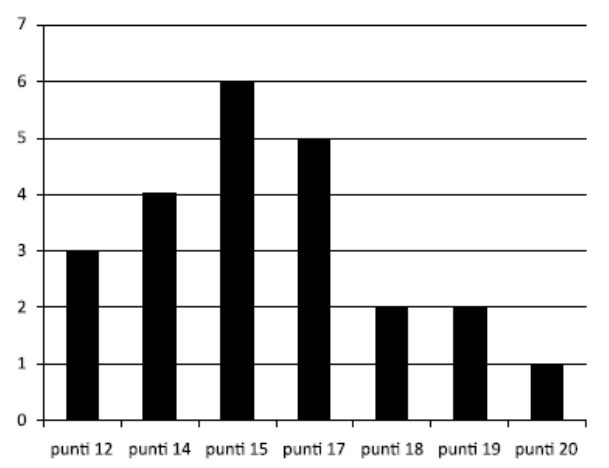
\includegraphics[width=0.75\textwidth]{images/istogramma_1.png}
\end{center}
\noindent
\vspace{0.5em}
Quante coppie hanno partecipato alla gara? \\
\begin{tabularx}{\linewidth}{@{}X X X X@{}}
\boxed{A}\hspace{6pt} 20 &
\boxed{B}\hspace{6pt} 23 &
\boxed{C}\hspace{6pt} 6 &
\boxed{D}\hspace{6pt} 115
\end{tabularx}

\vspace{15pt}

\noindent
Quante coppie hanno ottenuto almeno 15 punti? \\
\begin{tabularx}{\linewidth}{@{}X X X X@{}}
\boxed{A}\hspace{6pt} 10 &
\boxed{B}\hspace{6pt} 6 &
\boxed{C}\hspace{6pt} 13 &
\boxed{D}\hspace{6pt} 16
\end{tabularx}

\vspace{15pt}

\noindent
Quale è la moda nei punteggi ottenuti? \\
\begin{tabularx}{\linewidth}{@{}X X X X@{}}
\boxed{A}\hspace{6pt} 15 &
\boxed{B}\hspace{6pt} 17 &
\boxed{C}\hspace{6pt} 6 &
\boxed{D}\hspace{6pt} 16,42
\end{tabularx}
\begin{solution}
Leggere le barre dell'istogramma sommando le frequenze:
\begin{enumerate}
    \item Il totale delle coppie è la somma di tutte le frequenze → Risposta: \textbf{B} (23).
    \item Sommare le frequenze per punteggi $\ge 15$ → Risposta: \textbf{C} (13).
    \item La moda corrisponde alla barra più alta → Risposta: \textbf{A} (punteggio 15).
\end{enumerate}
\end{solution}
\end{question}

%----------------------------------------------------%

\begin{question}[ID=1.2, subtitle={Lettura di un diagramma a torta}, tags={torta}, difficulty=facile]
Il diagramma a torta mostra la situazione lavorativa di 500 laureati nel 2003.

\begin{center}
    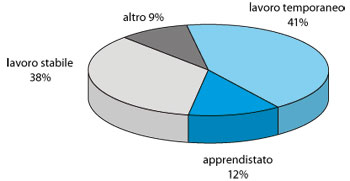
\includegraphics[width=0.55\textwidth]{images/grafico a torta.jpg}
\end{center}
\noindent
\vspace{0.5em}
Quanti laureati hanno un lavoro stabile? \\
\begin{tabularx}{\linewidth}{@{}X X X X@{}}
\boxed{A}\hspace{6pt} 131 &
\boxed{B}\hspace{6pt} 38 &
\boxed{C}\hspace{6pt} 380 &
\boxed{D}\hspace{6pt} 190
\end{tabularx}

\vspace{15pt}

\noindent
I laureati con lavoro stabile o apprendistato sono di più di coloro che hanno un lavoro temporaneo o altro?
\hfill
\begin{tabularx}{0.25\linewidth}{@{}X X@{}}
\boxed{VERO}&
\boxed{FALSO}
\end{tabularx}
\vspace{15pt}

\noindent
Si potrebbe migliorare la resa grafica del diagramma? E se sì, come?\vspace{10pt}\\
\rule{\linewidth}{0.2pt} \vspace{0.1pt} \\
\rule{\linewidth}{0.2pt} \vspace{0.1pt}
\begin{solution}
\begin{enumerate}
    \item La fetta «lavoro stabile» rappresenta il 38\% di 500 = 190 → Risposta: \textbf{D}.
    \item Dipende dai valori letti nel grafico; in genere la somma stabile+apprendistato supera temporaneo+altro → \textbf{VERO}.
    \item Sì: si potrebbe usare un istogramma o indicare esplicitamente le percentuali su ogni fetta.
\end{enumerate}
\end{solution}
\end{question}


%----------------------------------------------------%

\begin{question}[ID=1.3, subtitle={Grafici fuorvianti: scala dell'asse}, tags={istogramma, grafici fuorvianti}, difficulty=facile]
I seguenti grafici rappresentano lo stesso dato, il valore di un prodotto dal 2002 al 2022.

\begin{center}
    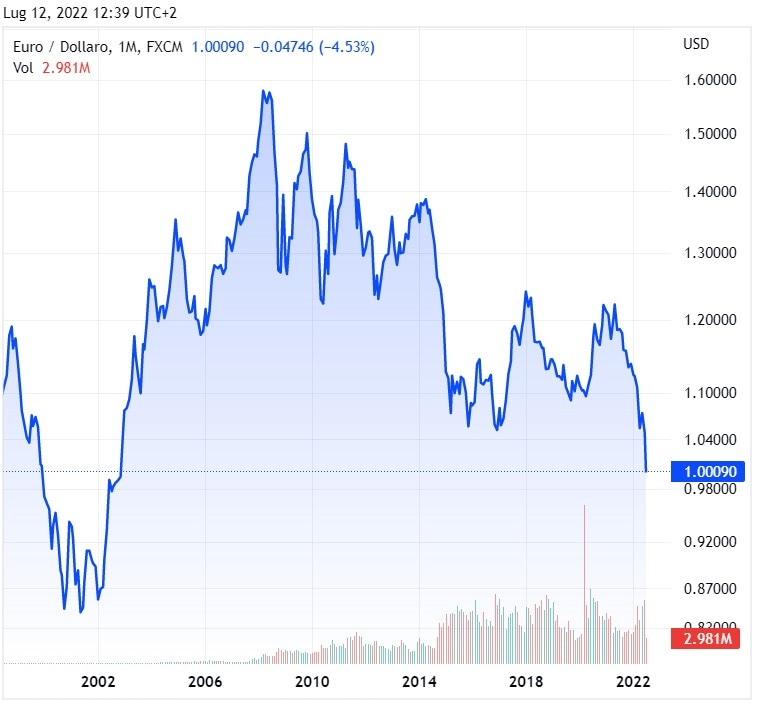
\includegraphics[width=0.45\textwidth]{images/cambio euro dollaro-2.jpg}
    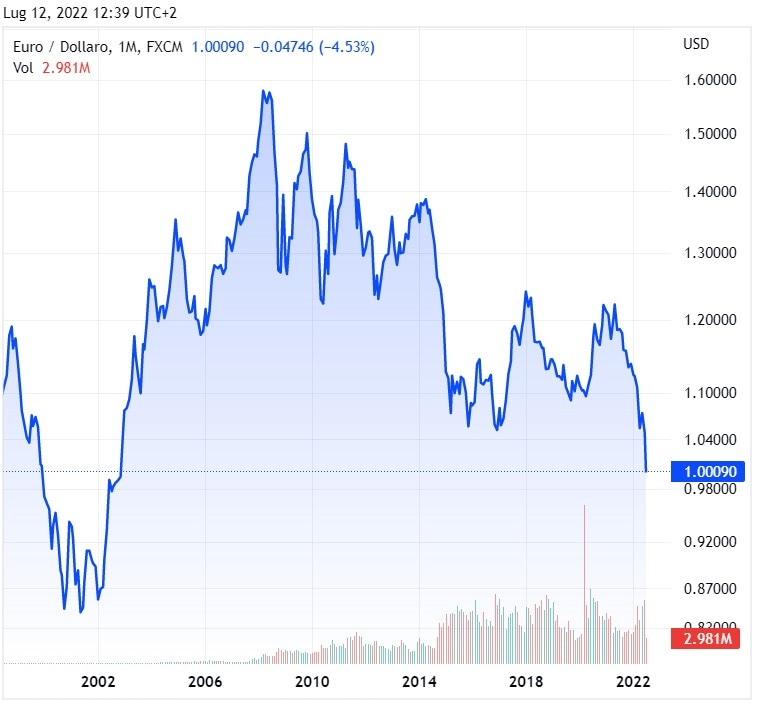
\includegraphics[width=0.45\textwidth, height=100pt]{images/cambio euro dollaro-2.jpg}
\end{center}
\noindent
In quale anno il valore ha raggiunto i suoi massimi?\\
\begin{tabularx}{\linewidth}{@{}X X X X@{}}
\boxed{A}\hspace{6pt} 2002 &
\boxed{B}\hspace{6pt} 2008 &
\boxed{C}\hspace{6pt} 2018 &
\boxed{D}\hspace{6pt} 2013
\end{tabularx}

\vspace{15pt}

\noindent
Rispetto all'inizio dei dati rappresentati, come è cambiato il valore nel 2022?\\
\begin{tabularx}{\linewidth}{@{}X X X X@{}}
\boxed{A}\hspace{6pt} É aumentato &
\boxed{B}\hspace{6pt} É diminuito &
\boxed{C}\hspace{6pt} É lo stesso &
\boxed{D}\hspace{6pt} Non si può dire
\end{tabularx}

\vspace{15pt}

\noindent
Quale tra i due grafici confonde di più? E perché?\vspace{10pt}\\
\rule{\linewidth}{0.2pt} \vspace{0.1pt} \\
\rule{\linewidth}{0.2pt} \vspace{0.1pt} \\
\rule{\linewidth}{0.2pt} \vspace{0.1pt} \\
\rule{\linewidth}{0.2pt} \vspace{0.1pt} \\
\begin{solution}
\begin{enumerate}
    \item Il massimo si trova intorno al 2008 → Risposta: \textbf{B}.
    \item Il valore nel 2022 è inferiore a quello del 2002 → Risposta: \textbf{B} (è diminuito).
    \item Il secondo grafico (con proporzioni alterate) confonde di più: comprimendo l'asse verticale le variazioni sembrano meno marcate di quanto non siano realmente.
\end{enumerate}
\end{solution}
\end{question}

%----------------------------------------------------%

\begin{question}[ID=1.4, subtitle={Lettura di ideogrammi con dati per paese}, tags={istogramma, grafici fuorvianti}, difficulty=facile]
Considera il seguente grafico che riporta i dati relativi al 2004 e controlla le affermazioni:
\begin{center}
    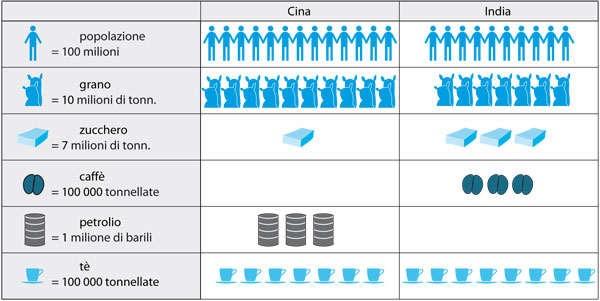
\includegraphics[width=0.75\textwidth]{images/idoegrammi.jpg}
\end{center}
\vspace{15pt}

\noindent
\color{gray}
In Cina vi erano 1 miliardo e 300 milioni di abitanti.
\hfill
\begin{tabularx}{0.25\linewidth}{@{}X X@{}}
\boxed{VERO}&
\boxed{FALSO}&
\end{tabularx}

\vspace{15pt}

\noindent
\color{black}
L'India ha prodotto 7 milioni di tonnellate di zucchero.
\hfill
\begin{tabularx}{0.25\linewidth}{@{}X X@{}}
\boxed{VERO}&
\boxed{FALSO}&
\end{tabularx}

\vspace{15pt}

\noindent
L'India ha prodotto 200.000 tonnellate in più di tè rispetto alla Cina.
\hfill
\begin{tabularx}{0.25\linewidth}{@{}X X@{}}
\boxed{VERO}&
\boxed{FALSO}&
\end{tabularx}

\vspace{15pt}

\noindent
Quale è il nome della tipologia di grafico utilizzato?
\hfill \rule{0.35\linewidth}{0.2pt}

\vspace{15pt}

\noindent
Come potresti manipolare il grafico per proporre una tua personale opinione?\vspace{10pt}\\
\rule{\linewidth}{0.2pt} \vspace{0.1pt} \\
\rule{\linewidth}{0.2pt} \vspace{0.1pt} \\
\rule{\linewidth}{0.2pt} \vspace{0.1pt} \\
\rule{\linewidth}{0.2pt} \vspace{0.1pt}
\begin{solution}
Leggere i valori direttamente dal grafico.
\begin{enumerate}
    \item Cina 1,3 miliardi di abitanti → \textbf{VERO}.
    \item India produzione zucchero: verificare la scala → risposta dipende dal grafico.
    \item India vs Cina per il tè: verificare la differenza leggendo le barre.
    \item Il grafico è un \textbf{ideogramma} (pictogram).
    \item Si potrebbe cambiare la scala dell'asse o scegliere selettivamente quali paesi confrontare.
\end{enumerate}
\end{solution}
\end{question}

%====================================================%
% SEZIONE 2: Istogramma delle frequenze, indici statistici
%====================================================%
\begin{question}[ID=2.1, subtitle={Indici statistici e istogramma del periodo di un pendolo}, tags={istogramma, indici statistici}, difficulty=media]
Un gruppo di studenti misura 10 volte il periodo di oscillazione di un pendolo, ottenendo i seguenti tempi in secondi:
\begin{center}
    10,1 \qquad 10,4 \qquad 9,5 \qquad 10,2 \qquad 10,1 \qquad 9,6 \qquad 10,0 \qquad 9,6 \qquad 10,4 \qquad 10,1
\end{center}

\noindent
Determinare:
\begin{enumerate}
    \item Il valor medio, la moda, la mediana, la varianza e lo scarto quadratico medio \\
     \framebox(\linewidth,250){}
    \item la tabella delle frequenze e l'istogramma delle frequenza realizzando classi di ampiezza $0{,}3\ \text{s}$\\
     \framebox(\linewidth,250){}
\end{enumerate}
\begin{solution}
Dati ordinati: 9,5 — 9,6 — 9,6 — 10,0 — 10,1 — 10,1 — 10,1 — 10,2 — 10,4 — 10,4.
\begin{enumerate}
    \item
    \begin{itemize}
        \item Media: $\bar{x} = (9{,}5+9{,}6+9{,}6+10{,}0+10{,}1+10{,}1+10{,}1+10{,}2+10{,}4+10{,}4)/10 = 100{,}0/10 = 10{,}00\ \text{s}$.
        \item Moda: $10{,}1\ \text{s}$ (compare 3 volte).
        \item Mediana: media dei valori centrali: $(10{,}1+10{,}1)/2 = 10{,}1\ \text{s}$.
        \item Varianza: $\sigma^2 = \frac{1}{n}\sum(x_i-\bar{x})^2 \approx 0{,}082\ \text{s}^2$.
        \item Scarto quadratico medio: $\sigma \approx 0{,}29\ \text{s}$.
    \end{itemize}
    \item Classi di ampiezza 0,3 s: [9,4–9,7): 3; [9,7–10,0): 1; [10,0–10,3): 4; [10,3–10,6): 2.
\end{enumerate}
\end{solution}
\end{question}
